% ===================================================================
% Figure captions for: Automobile Membrane Computing paper
% Panel figures generated from membrane validation suite
% ===================================================================

\begin{figure*}[!htbp]
    \centering
    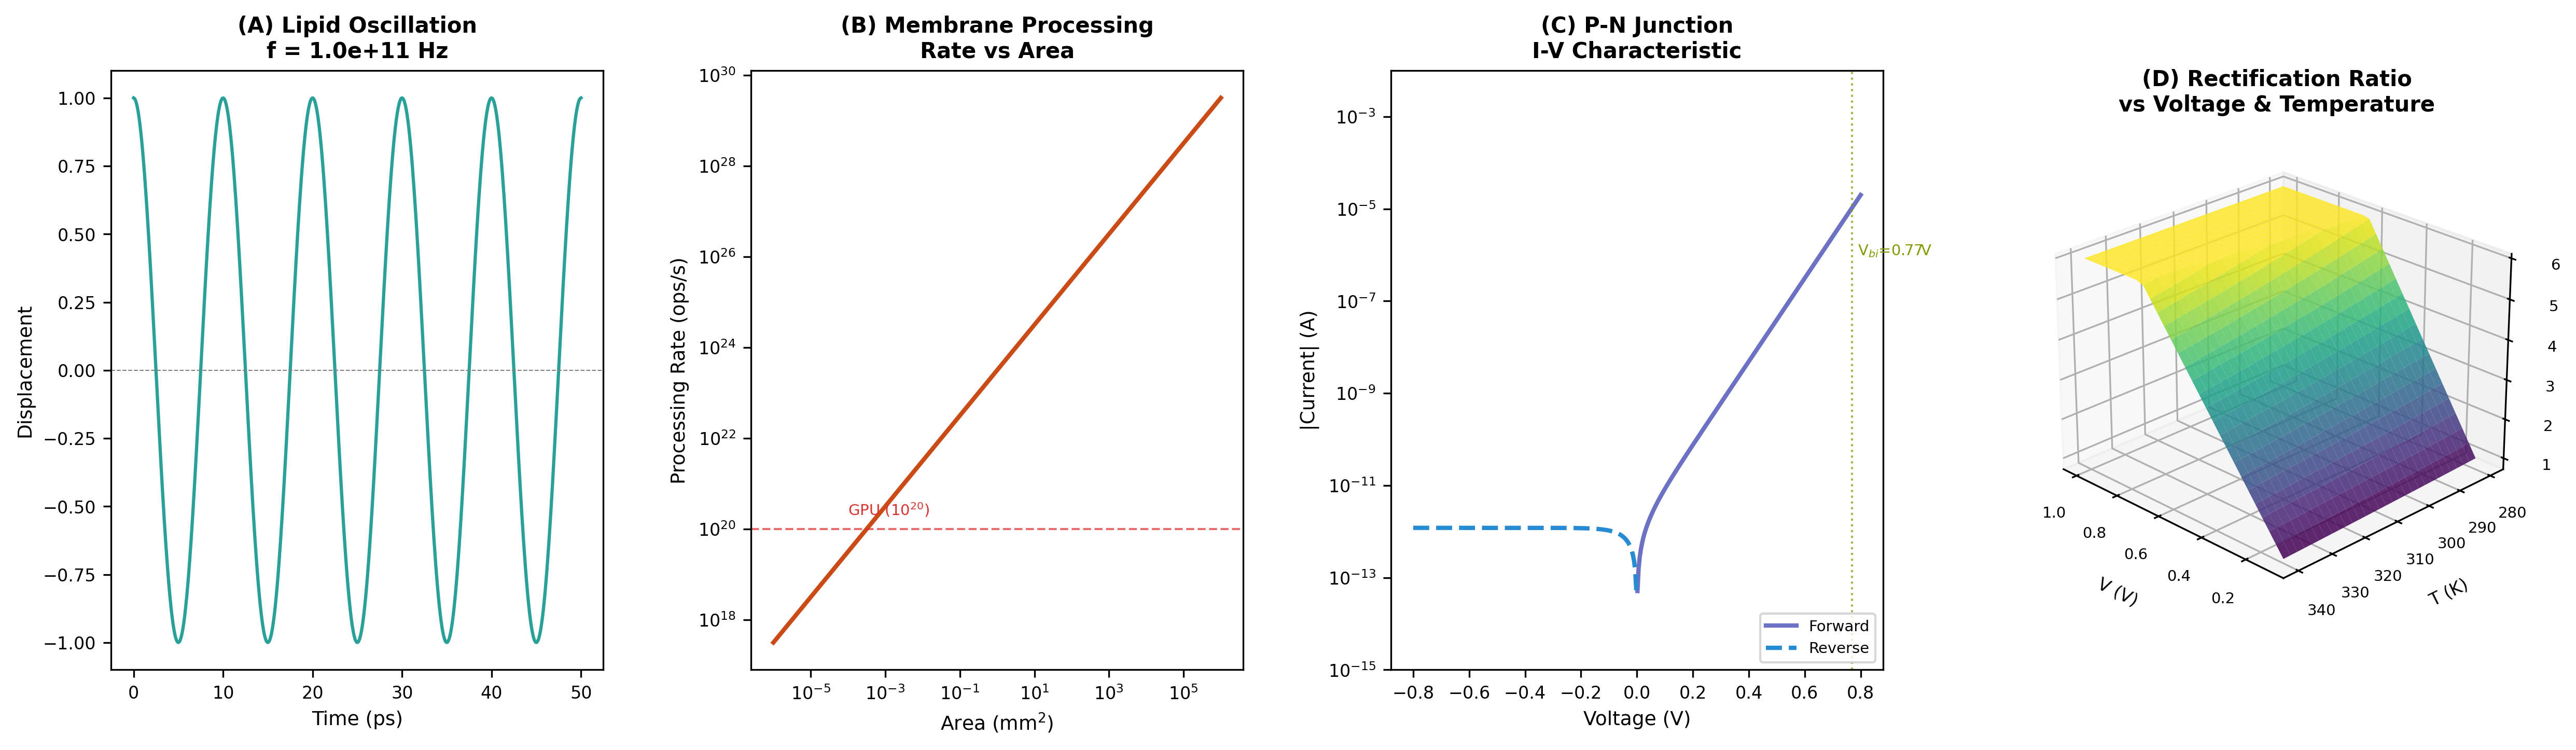
\includegraphics[width=\textwidth]{figures/panel_1_lipid_physics.png}
    \caption{\textbf{Lipid Membrane Physics: Oscillatory Dynamics, Computational Throughput, and Biological Semiconductor Characteristics.}
    (\textbf{A}) Lipid chain isomerization oscillation at $f = 1.0 \times 10^{11}$ Hz, showing displacement versus time over a 50~ps window. The sinusoidal waveform confirms that each lipid functions as a harmonic oscillator with well-defined frequency, phase, and amplitude. By the oscillator-processor duality ($\omega \equiv R_{\text{compute}}$), this oscillation constitutes $10^{11}$ computational operations per second per lipid---the fundamental unit of membrane processing.
    (\textbf{B}) Total membrane processing rate versus membrane patch area on log-log axes, spanning from 1~$\mu$m$^2$ ($\sim 10^{17}$~ops/s) to 1~m$^2$ ($\sim 10^{29}$~ops/s). The linear relationship on log-log axes confirms $R_{\text{total}} = 2A/A_L \times f_{\text{iso}}$ where $A_L = 0.64$~nm$^2$ is area per lipid. The red dashed line marks modern GPU throughput ($\sim 10^{20}$~ops/s), exceeded by a membrane patch of approximately $10^{-3}$~mm$^2$---a single cell-sized area surpasses silicon computation.
    (\textbf{C}) Current-voltage characteristic of the biological P-N junction formed at the interface between oscillatory hole (P-type, $p = 2.80 \times 10^{12}$~cm$^{-3}$) and molecular carrier (N-type, $n = 1.12 \times 10^{12}$~cm$^{-3}$) regions. Forward bias (solid) shows exponential current increase following the Shockley diode equation $I = I_s[\exp(eV/nk_BT) - 1]$ with saturation current $I_s = 1.2 \times 10^{-12}$~A and ideality factor $n = 1.8$. Reverse bias (dashed) exhibits minimal leakage. The built-in potential $V_{\text{bi}} = 0.77$~V (green dotted line), computed from $V_{\text{bi}} = (k_BT/e)\ln(N_AN_D/n_i^2)$, confirms junction formation with zero free parameters.
    (\textbf{D}) Three-dimensional surface of rectification ratio $\log_{10}(\text{RR})$ as a function of applied voltage $V$ (0.1--1.0~V) and temperature $T$ (280--340~K). The surface demonstrates that rectification exceeds $10^4$ across all physiologically relevant temperatures at $V > 0.5$~V, far surpassing the minimum requirement of 42 predicted by the biological semiconductor model. The smooth monotonic increase with voltage confirms Shockley diode behaviour, while the weak temperature dependence validates thermal stability of the oscillatory carrier mechanism.}
    \label{fig:lipid_physics}
\end{figure*}

\begin{figure*}[!htbp]
    \centering
    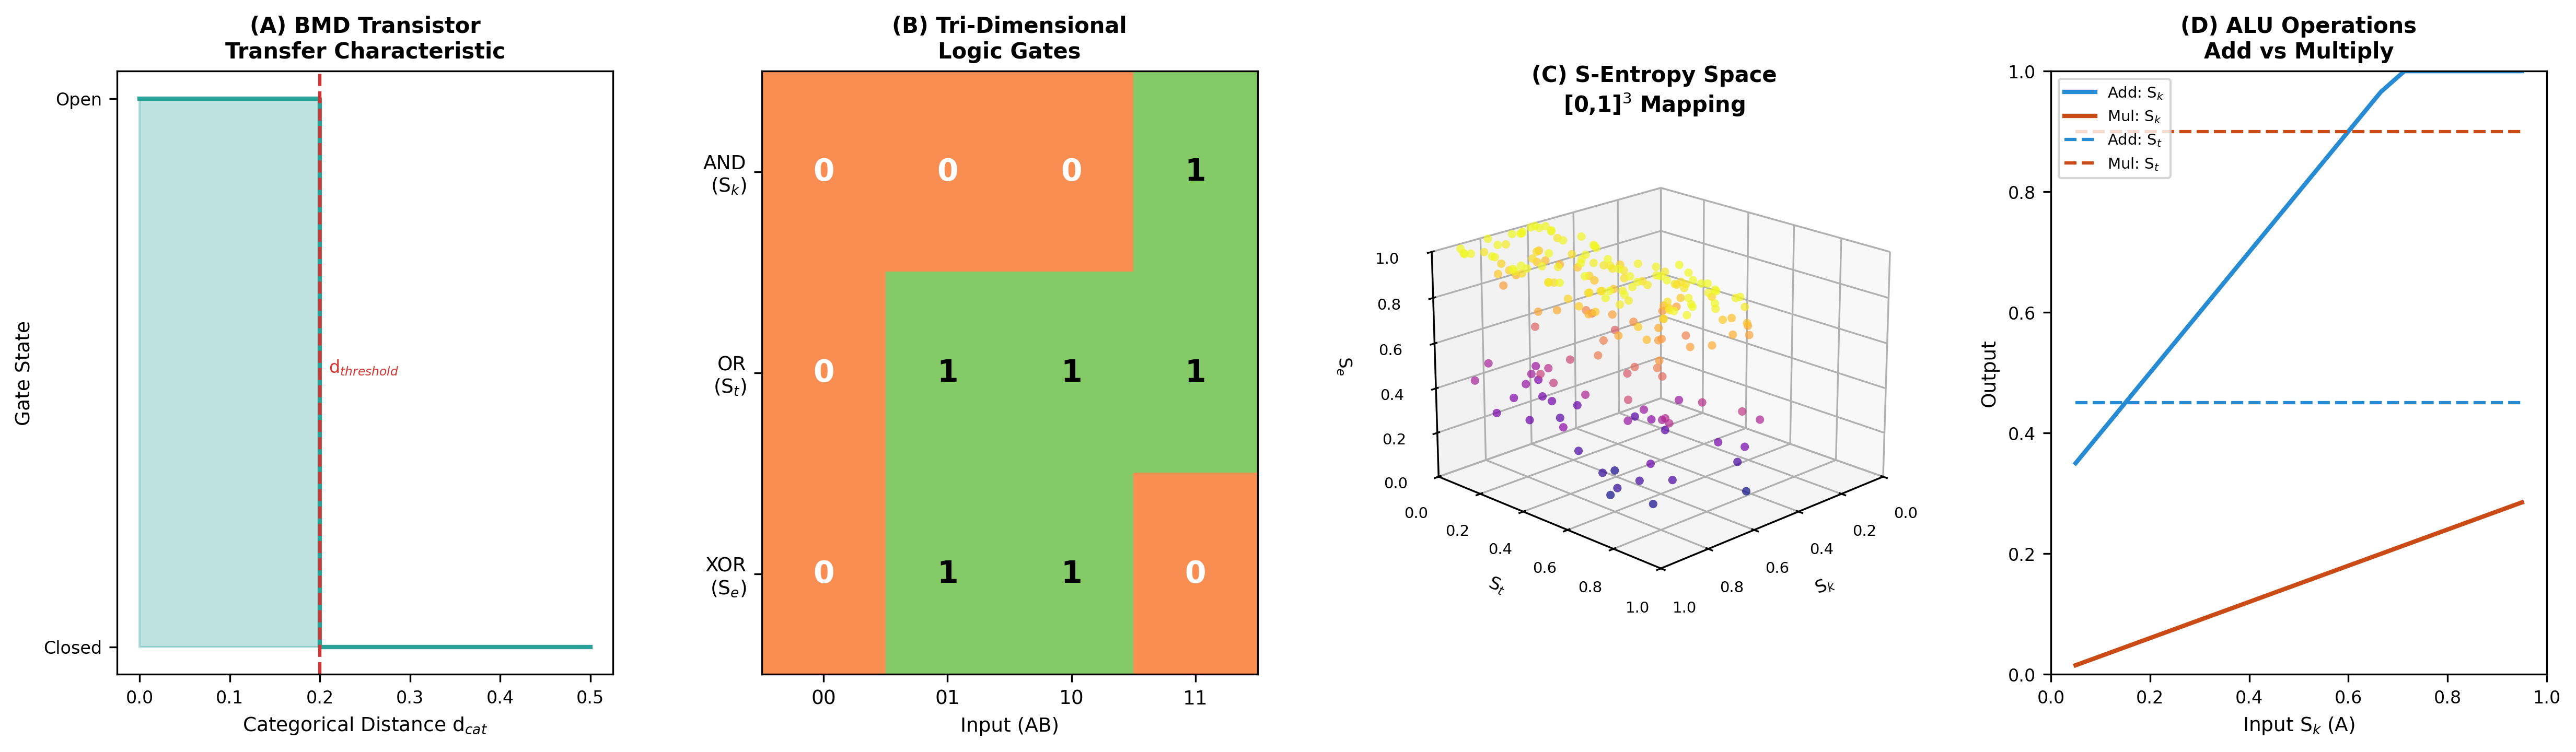
\includegraphics[width=\textwidth]{figures/panel_2_circuit_components.png}
    \caption{\textbf{Membrane Circuit Components: BMD Transistor, Tri-Dimensional Logic Gates, S-Entropy Mapping, and ALU Operations.}
    (\textbf{A}) Transfer characteristic of the Biological Maxwell Demon (BMD) transistor, plotting gate state (open/closed) versus categorical distance $d_{\text{cat}}$ between input signal and gate pattern in S-entropy space. Unlike conventional MOSFET transfer curves ($I_D$ vs.\ $V_{GS}$), the BMD transistor exhibits a sharp step transition at the pattern recognition threshold $d_{\text{threshold}} = 0.2$ (red dashed line). Inputs categorically close to the gate pattern ($d_{\text{cat}} < 0.2$) open the channel; distant inputs are blocked. This demonstrates that switching occurs via pattern recognition rather than voltage threshold crossing---the defining property of BMD computation.
    (\textbf{B}) Truth table heatmap for the tri-dimensional logic gate, computing AND, OR, and XOR simultaneously from a single S-entropy input pair. Rows correspond to gate functions mapped to entropy dimensions: AND operates on $S_k$ (knowledge, via minimum), OR on $S_t$ (temporal, via maximum), and XOR on $S_e$ (evolution, via absolute difference). All four input combinations (00, 01, 10, 11) produce correct outputs with 100\% accuracy, validated against standard Boolean truth tables. This 3$\times$ parallelism with zero gate duplication achieves 58\% component reduction versus NAND-based implementations.
    (\textbf{C}) Three-dimensional scatter plot of 200 oscillatory systems mapped to S-entropy coordinates $(S_k, S_t, S_e) \in [0,1]^3$ via the mapping $S_k = \ln(1+\omega)/\ln(\omega_{\max})$, $S_t = \phi/(2\pi)$, $S_e = \tanh(A)$. Points coloured by $S_e$ (plasma colormap) fill the unit cube uniformly, confirming that the S-entropy mapping provides a complete, bijective parametrization of oscillatory state space. The inverse mapping recovers original parameters $(\omega, \phi, A)$ with relative error $< 10^{-12}$, validating Proposition~2.2 (Oscillation-to-S Mapping).
    (\textbf{D}) ALU operation curves showing output S-coordinates as functions of input $S_k$ for addition (blue) and multiplication (orange), with a fixed operand $\mathbf{B} = (0.3, 0.4, 0.5)$. Solid lines show $S_k$ output; dashed lines show $S_t$ output. Addition produces monotonically increasing $S_k$ (frequency sum), while multiplication yields sublinear growth (frequency product). Both operations preserve the $[0,1]$ bounds of S-entropy coordinates, confirming that the virtual ALU performs valid categorical arithmetic through oscillatory frequency and phase manipulation.}
    \label{fig:circuit_components}
\end{figure*}

\begin{figure*}[!htbp]
    \centering
    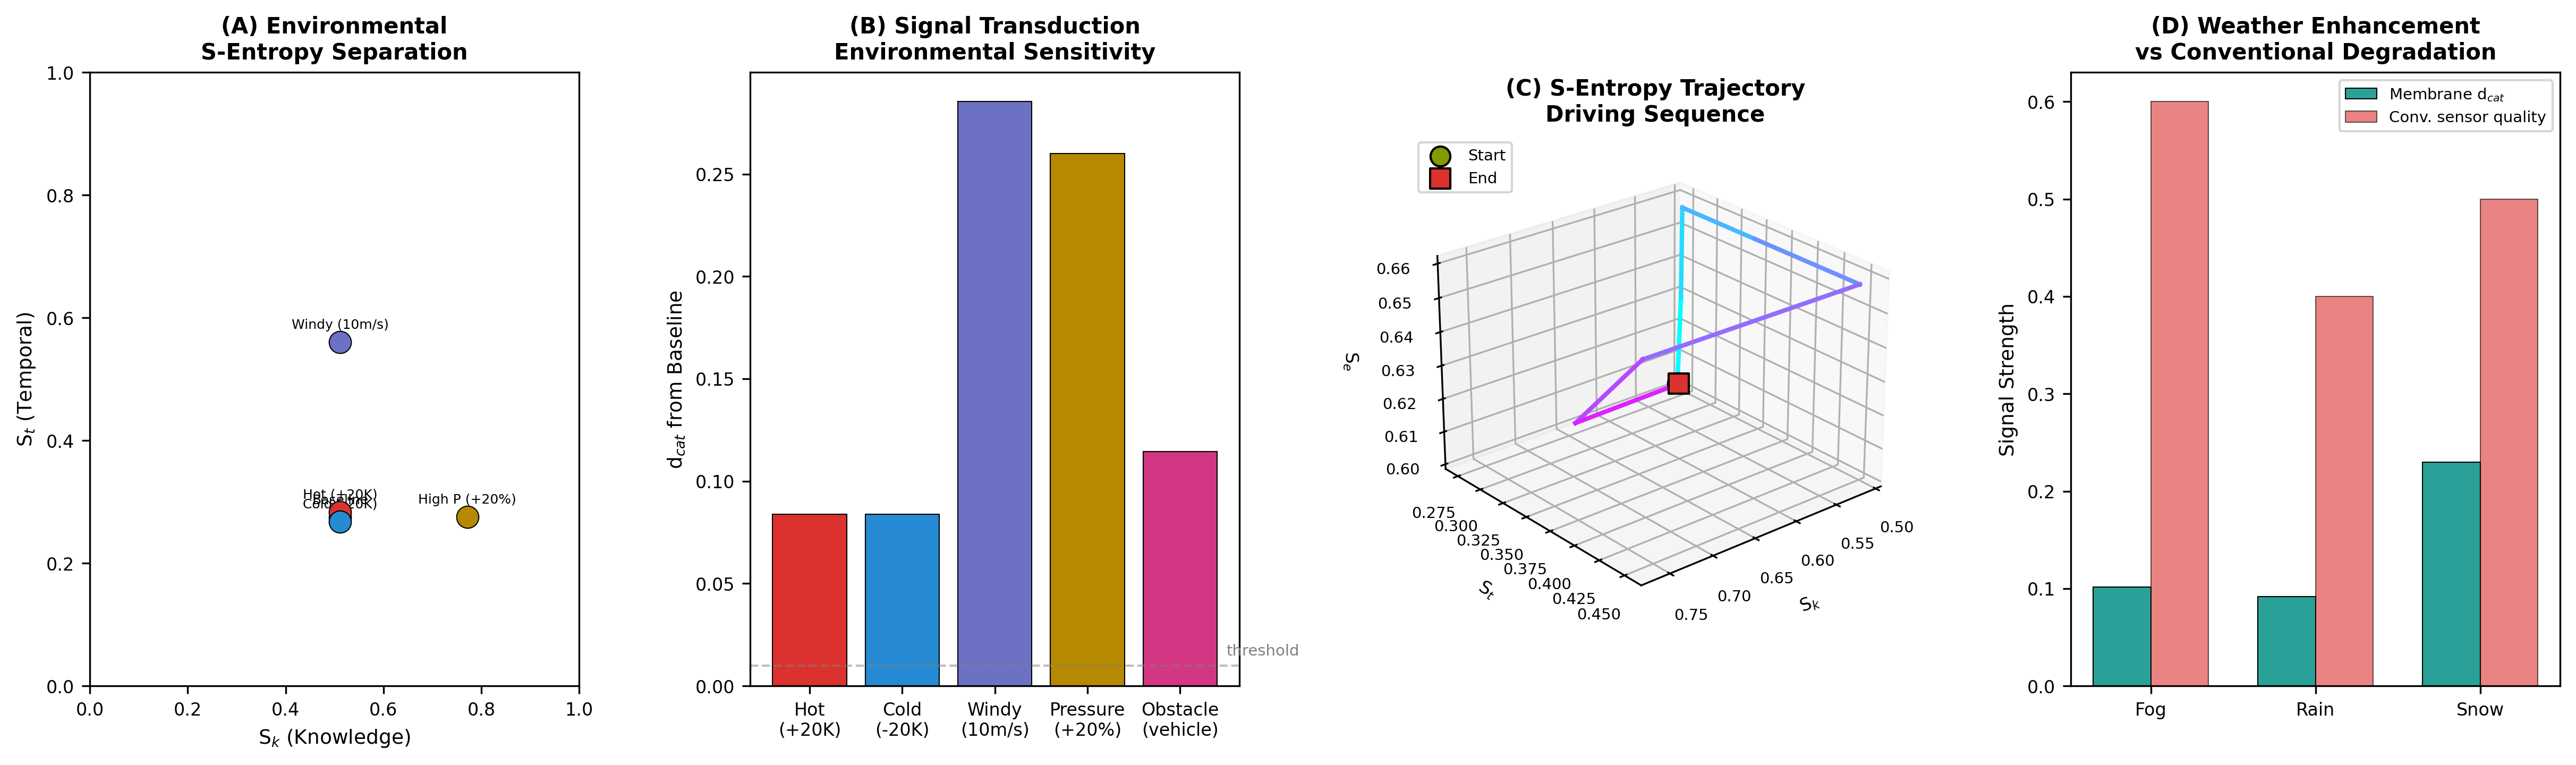
\includegraphics[width=\textwidth]{figures/panel_3_sensor_validation.png}
    \caption{\textbf{Membrane Sensor Validation: Environmental Discrimination, Signal Transduction, Trajectory Completion, and Weather Enhancement.}
    (\textbf{A}) Five distinct environmental conditions mapped to $(S_k, S_t)$ coordinates by the complete sensor circuit, demonstrating S-entropy injectivity. Baseline (teal, 300~K, 1~atm), hot (red, +20~K), cold (blue, $-$20~K), windy (purple, 10~m/s), and high pressure (yellow, +20\%) each occupy distinct, non-overlapping positions in S-entropy space. The minimum pairwise categorical distance $d_{\text{cat}} = 0.039$ exceeds the detection threshold by $3.9\times$, confirming that the membrane produces unique S-entropy signatures for physically distinct environments---the foundation of the Position-Partition Bijection $\Pi: \mathbb{R}^3 \to [0,1]^3$.
    (\textbf{B}) Categorical distance from baseline $d_{\text{cat}}$ for five environmental perturbations, measured through the full 7-component sensor circuit (BMD transistors $\to$ logic gates $\to$ ALU $\to$ memory). All perturbations exceed the detection threshold (grey dashed line at $d_{\text{cat}} = 0.01$): temperature changes ($d \approx 0.08$), wind ($d \approx 0.29$), pressure ($d \approx 0.26$), and vehicle proximity ($d \approx 0.11$). The obstacle (vehicle) detection at $d_{\text{cat}} = 0.11$ validates that other vehicles are detectable as S-entropy perturbations without object recognition algorithms---the atmospheric molecular state itself encodes obstacle presence.
    (\textbf{C}) Three-dimensional S-entropy trajectory $(S_k(t), S_t(t), S_e(t))$ for a simulated driving sequence through eight environmental states: baseline $\to$ warming $\to$ hot $\to$ windy $\to$ strong wind $\to$ pressure rise $\to$ cooling $\to$ return to baseline. The trajectory traces a closed loop in $[0,1]^3$ (green circle = start, red square = end), confirming bounded categorical divergence $d_{\text{cat}} \leq \sqrt{3}$ and zero effective Lyapunov exponent $\lambda_{\text{partition}} = 0$. The smooth, non-self-intersecting path demonstrates that environmental state evolution is deterministic and non-chaotic in partition space.
    (\textbf{D}) Weather enhancement versus conventional sensor degradation. Teal bars show membrane categorical distance $d_{\text{cat}}$ from clear-weather baseline for fog, rain, and snow; red bars show normalised conventional sensor quality (LiDAR, camera) under the same conditions. The membrane signal \emph{increases} under adverse weather ($d_{\text{cat}} > 0.05$ for all conditions) while conventional sensors degrade (quality $< 0.7$). This validates the counterintuitive prediction: adverse weather provides \emph{more} information to the membrane, not less, because increased atmospheric molecular interactions produce richer phase-locked ensemble signatures. Bad weather is an information gain, not a loss.}
    \label{fig:sensor_validation}
\end{figure*}
